\documentclass{article}

\usepackage{hyperref}
\usepackage{amsmath}
\usepackage{graphicx}
\usepackage{subcaption}
\usepackage{epstopdf}
\usepackage{bm}

\usepackage{times}

% Page layout
\hoffset -0in
\voffset -1in
\oddsidemargin 0in
\textheight 9.3in
\textwidth 6.3in

\setlength{\parindent}{0pt}
\setlength{\intextsep}{5pt}
%\pagestyle{empty}

\graphicspath{{figures/}}

\begin{document}
	\section*{COMPUTATIONAL METHODS IN MECHANICS: Task 4}
	Vesa-Ville Hurskainen, 14 Feb 2018\\
	\href{https://github.com/VesaVilleHurskainen/cmim2018}{GitHub repository}

	\section*{Introduction}
	This is a report of the fourth assignment of the course \textit{Computational Methods in Mechanics}, concerning numerical integration applied to a three-spring-three-mass system. The assignment consists of six tasks, which are as follows:
	
	\begin{enumerate}
		\setlength\itemsep{0pt}
		\item To write the equations of motion for the three-mass-three-spring system.
		\item To numerically calculate the system's natural frequencies.
		\item To investigate how removing the first spring affects the natural frequencies.
		\item To solve the system with nonzero initial conditions using four solvers (odeRK4, odeSIE, ode45, ode15s) and compare accuracy and
		efficiency.
		\item To repeat the computations using nodal coordinates and compare the results with the original system.
		\item To write a report.
	\end{enumerate}

	\section*{Methods}
	Using Newton's second law, we can derive the following system of equations of motion for the three-mass system: 
	\begin{equation}
		\begin{aligned}
		m_1 \ddot{x}_1 & = - x_1 k_1 + (x_2 - x_1) k_2 \\
		m_2 \ddot{x}_2 & = - (x_2 - x_1) k_2 + (x_3 - x_2) k_3\\
		m_3 \ddot{x}_3 & = - (x_3 - x_2) k_3
		\end{aligned}
	\end{equation}
	Transforming the system of linear equations into matrix form, we get the matrix equation:
	\begin{equation}
		\mathbf{M} \ddot{\bm{x}} + \mathbf{K} \bm{x} = \bm{0}
	\end{equation}
	where the mass matrix $\mathbf{M}$ and stiffness matrix $\mathbf{K}$ are written as:
	\begin{equation}
		\begin{aligned}
		\mathbf{M} &= \text{diag}(m_1, m_2, m_3) \\
		\mathbf{K} &= \begin{bmatrix}
		k_1 + k_2 & -k_2 & 0 \\
		-k_2 & k_2 + k_3 & - k_3 \\
		0 & -k_3 & k_3
		\end{bmatrix}
		\end{aligned}
	\end{equation}
	The system was solved and the results plotted using the script \texttt{assignment4.m}. The previously-made function \texttt{formatPlot.m} was used to format the figures for printing. The function \texttt{testSolvers.m} was written to test the solvers and complete the preliminary hands-on part of the assignment.
	
	\section*{Results}
	The parameters for the system were given as follows: $m_1 = 2$ kg, $m_2 = 1.5$ kg, $m_3 = 1$ kg, $k_1 = 20,000$ N/m, $k_2 = 15,000$ N/m, $k_3 = 10,000$ N/m. The initial condition of $x_3 = 0.1$ was used to give the system an excitation. The numerical integration was performed using the following settings: $\Delta t = 0.001$ s, $t = 0 \dots 1$ s. The numerically calculated natural frequencies of the original and modified system are presented in Table~\ref*{tab:natural_frequencies}.
	
	\begin{table}[h!]
		\centering
		\begin{tabular}{|r|r|}
			\hline
			Original system & Modified: $k_1 = 0$ \\
			\hline
			51.08 rad/s & 0 rad/s \\
			117.5 rad/s & 94.38 rad/s \\
			166.6 rad/s & 158.9 rad/s \\
			\hline
		\end{tabular}
		\caption{Numerically computed natural frequencies of the system.}
		\label{tab:natural_frequencies}
	\end{table}

	\clearpage
	As an example of code output, Figure~\ref*{fig:assignment_rungekutta} presents the response computed using the Runge-Kutta 4th order method. Table~\ref*{tab:solver_comparison} compares the responses computed using different solvers. The reference result set was computed using the Runge-Kutta 4th order method with a very small time step ($\Delta t = $ 1e-6 s).

	\begin{figure}[h!]
		\centering
		\begin{subfigure}[t]{0.45\textwidth}
			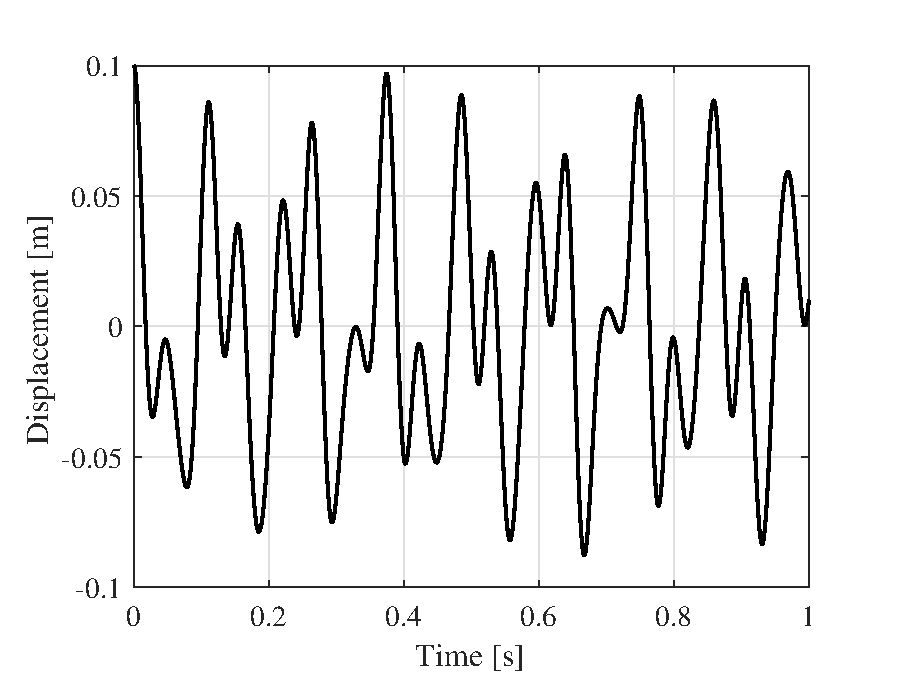
\includegraphics[width=\textwidth]{assignment_rk4_response.eps}
			\caption{Displacement of mass 3 vs. time.}
		\end{subfigure}~
		\begin{subfigure}[t]{0.45\textwidth}
			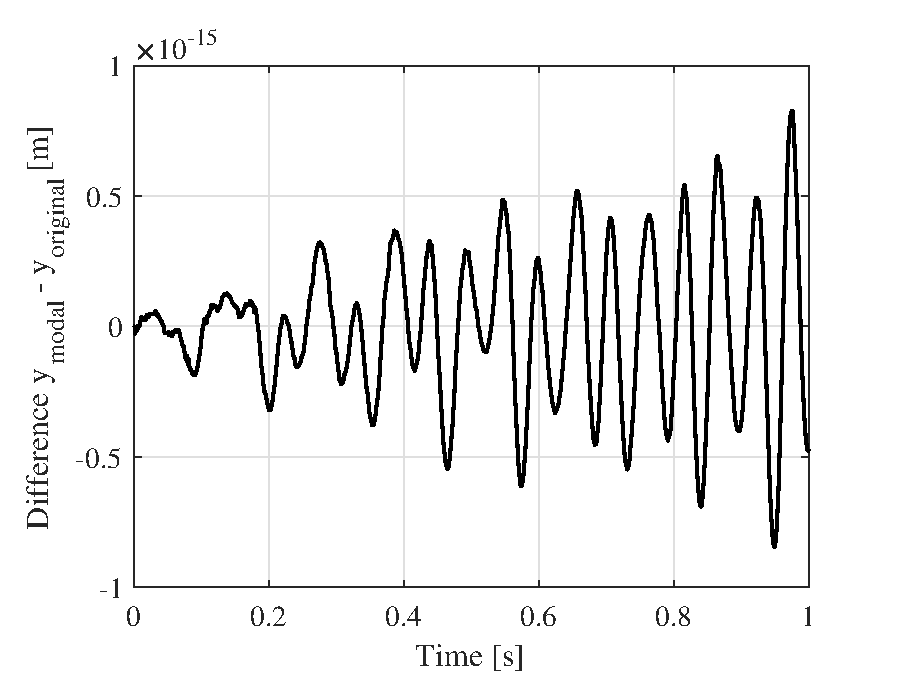
\includegraphics[width=\textwidth]{assignment_rk4_difference.eps}
			\caption{Difference between responses: original system / modal coordinate transformation.}
		\end{subfigure}\\
		\begin{subfigure}[t]{0.45\textwidth}
			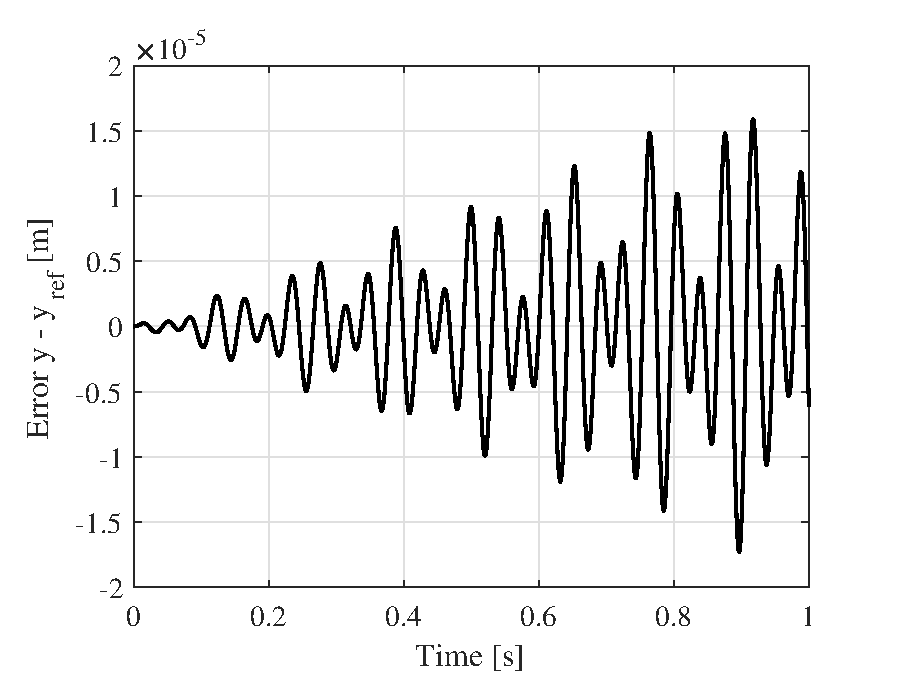
\includegraphics[width=\textwidth]{assignment_rk4_error.eps}
			\caption{Displacement error of mass 3 vs. time.}
		\end{subfigure}~
		\begin{subfigure}[t]{0.45\textwidth}
			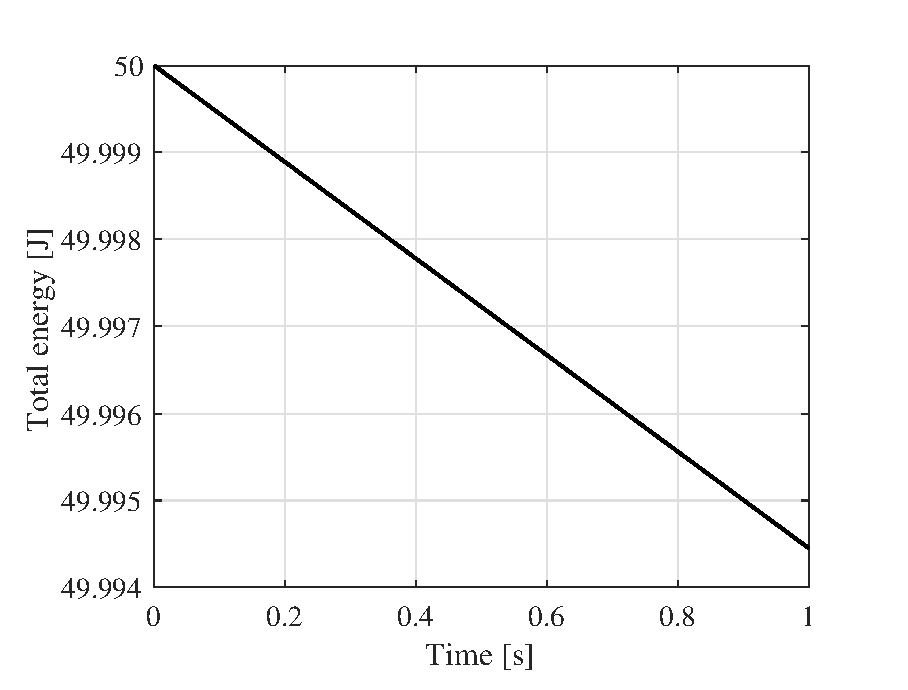
\includegraphics[width=\textwidth]{assignment_rk4_energy.eps}
			\caption{System energy vs. time.}
		\end{subfigure}
		\caption{Three-spring-three-mass system response with Runge-Kutta fourth order method.\label{fig:assignment_rungekutta}}
	\end{figure}

	\begin{table}[h!]
	\centering
	\begin{tabular}{|r|r|r|}
		\hline
		Solver & Max. disp. error & Max. energy drift \\
		\hline
		\texttt{rungeKutta4.m} & 17.3 nm & 0.00555 J\\
		\texttt{simEuler.m} & 8390 nm & 3.17 J\\
		\texttt{ode45} & 276 nm & 0.200 J\\
		\texttt{ode15s} & 1340 nm & 1.30 J\\
		\hline
	\end{tabular}
	\caption{Comparison of displacement errors and energy drifts when using different solvers.}
	\label{tab:solver_comparison}
	\end{table}

	\section*{Analysis}
	As Table~\ref*{tab:natural_frequencies} shows, the first natural frequency of the system goes to zero when the first spring is removed. This was expected, since doing so removes all stiffness constricting the system's movement in relation to the reference frame. The other two natural frequencies are also lowered; an expected result of reduced stiffness.\\
	
	As we can see from the results presented in Figure~\ref*{fig:assignment_rungekutta}, the difference between the responses of the original system and the modal coordinate transformation is small enough to likely result from the inaccuracies of floating point arithmetic. Table~\ref*{tab:solver_comparison} shows that the Runge-Kutta method shows the smallest error and energy drift and the semi-implicit euler the largest. The efficiency of self-written routines is difficult to compare to MATLAB solvers \texttt{ode45} and \texttt{ode15s}, since they choose the computational time step internally and only allow the user to set the maximum.
	
	\clearpage
	\section*{Preliminary hands-on task}
	\vspace{-1ex}
	\textbf{Forward Euler method}
	
	Function \texttt{[t,y] = fwdEuler(fun, tspan, y0)}: population in Fig.~\ref*{fig:fwdeuler_population}, mass-spring system results Fig.~\ref*{fig:fwdeuler_mass_spring}.
	
	\begin{figure}[h!]
		\centering
		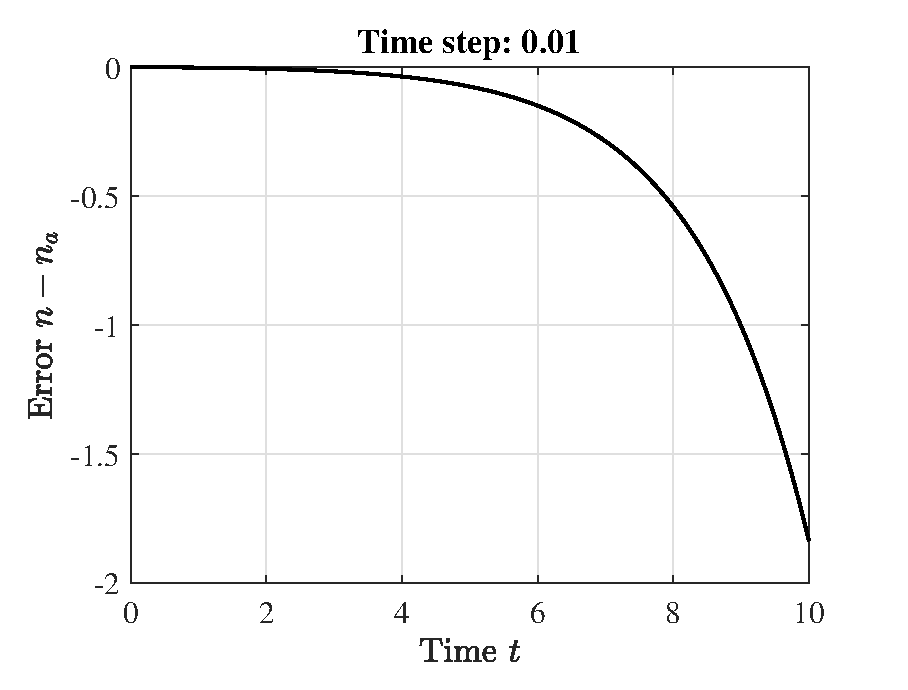
\includegraphics[width=0.33\textwidth]{fwdeuler_error1.eps}
		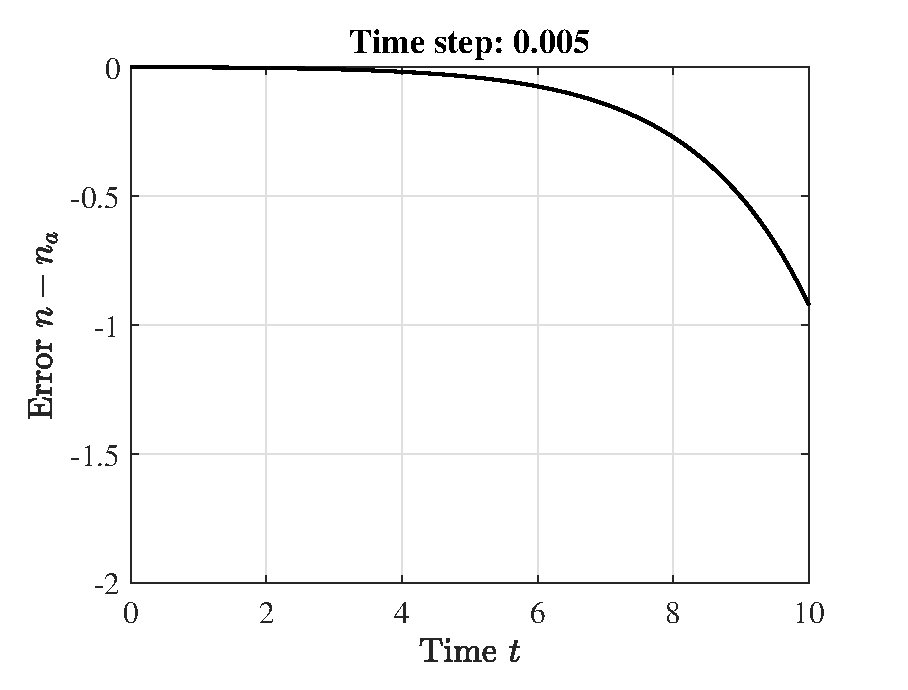
\includegraphics[width=0.33\textwidth]{fwdeuler_error2.eps}
		\caption{Population model error with forward Euler method, $r = 0.5$, $n_0 = 1$.\label{fig:fwdeuler_population}}
	\end{figure}
	\vspace{-1ex}
	\begin{figure}[h!]
		\centering
		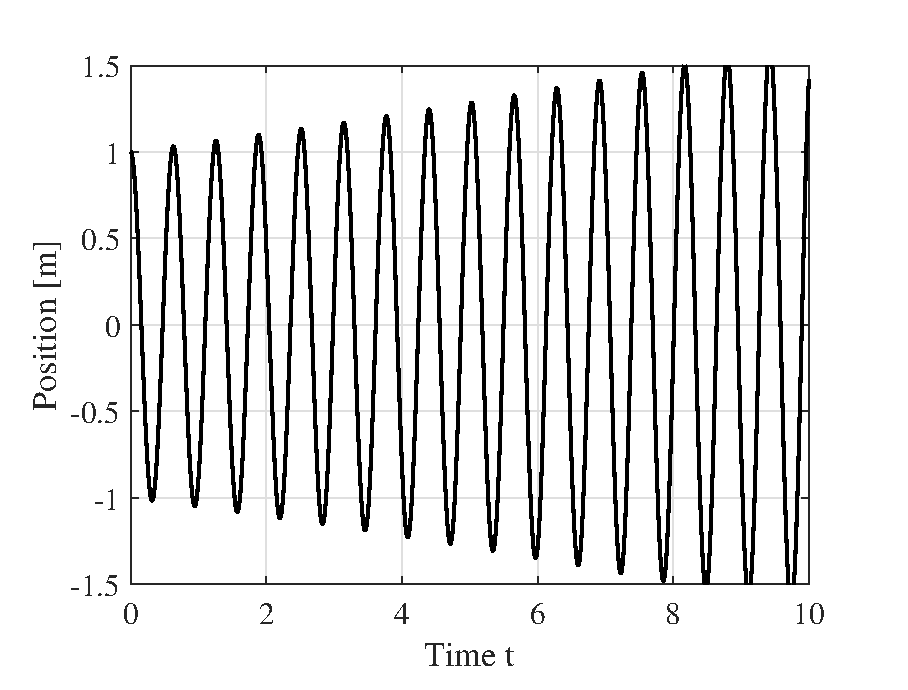
\includegraphics[width=0.33\textwidth]{fwdeuler_position.eps}
		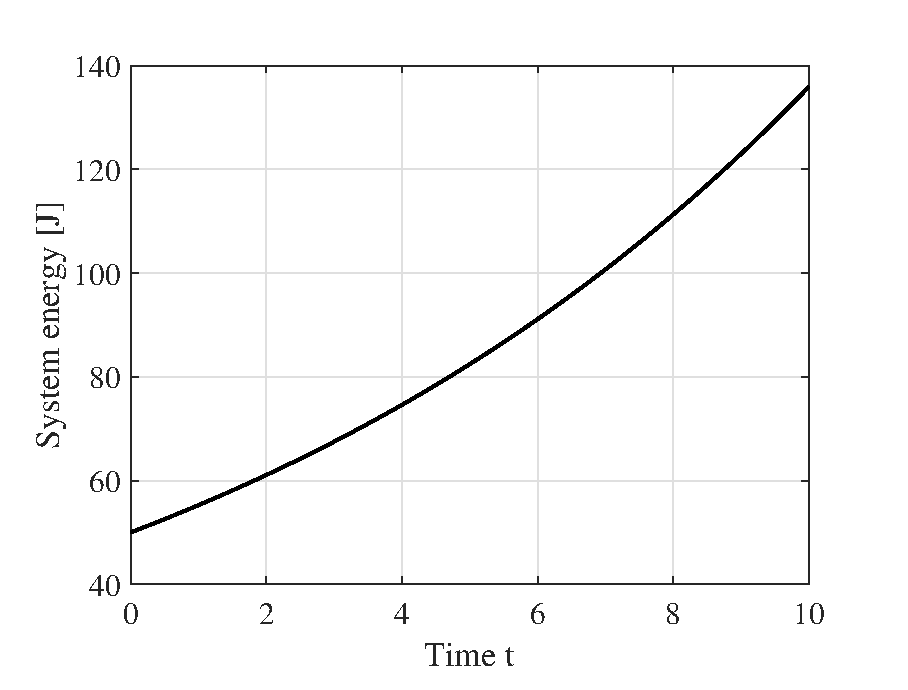
\includegraphics[width=0.33\textwidth]{fwdeuler_energy.eps}
		\caption{Mass-spring system with forward Euler method, $\Delta t = 0.001$ s, $m = 1$ kg, $k = 100$ N/m, $A = 1$ m.\label{fig:fwdeuler_mass_spring}}
	\end{figure}
	
	\textbf{Semi-implicit Euler method}
	
	Function \texttt{[t,u,v] = simEuler(fun\_f, fun\_g, tspan, u0, v0)}: mass-spring system results in Fig.~\ref*{fig:simeuler_mass_spring}.
	
	\begin{figure}[h!]
		\centering
		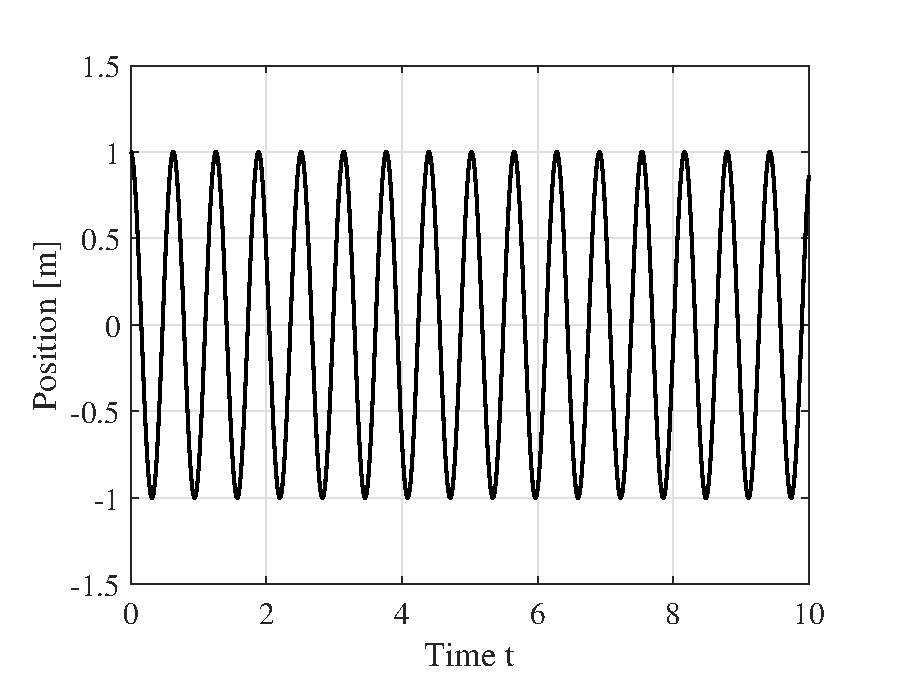
\includegraphics[width=0.33\textwidth]{simeuler_position.eps}
		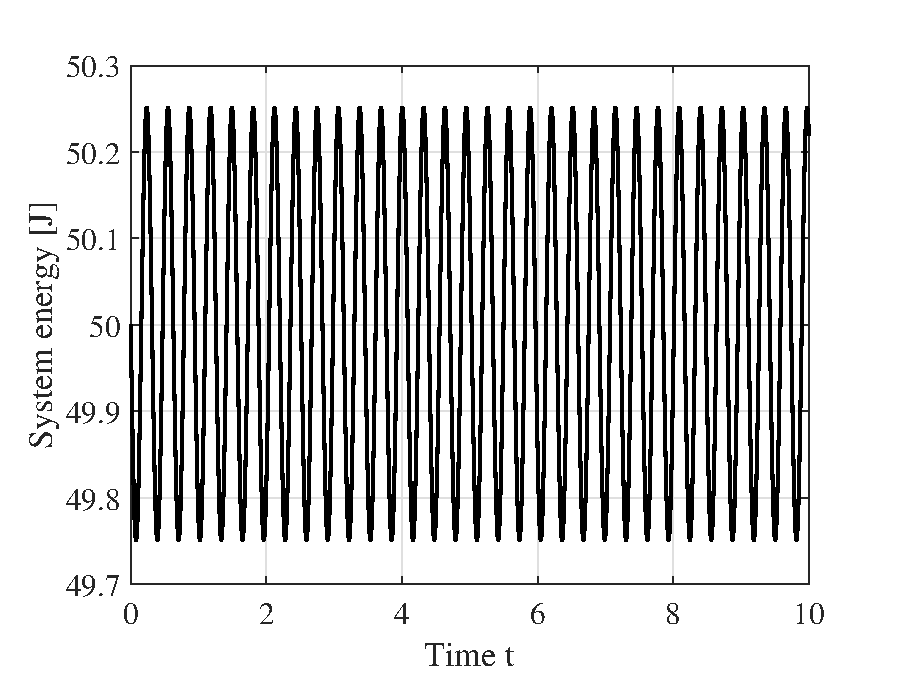
\includegraphics[width=0.33\textwidth]{simeuler_energy.eps}
		\caption{Mass-spring system with semi-implicit Euler method, $\Delta t = 0.001$ s $m = 1$ kg, $k = 100$ N/m, $A = 1$ m.\label{fig:simeuler_mass_spring}}
	\end{figure}
	
	\textbf{Runge-Kutta method}
	
	Function \texttt{[t,y] = rungeKutta4(fun, tspan, y0)}: mass-spring system results in Fig.~\ref*{fig:rungekutta_mass_spring}.
	
	\begin{figure}[h!]
		\centering
		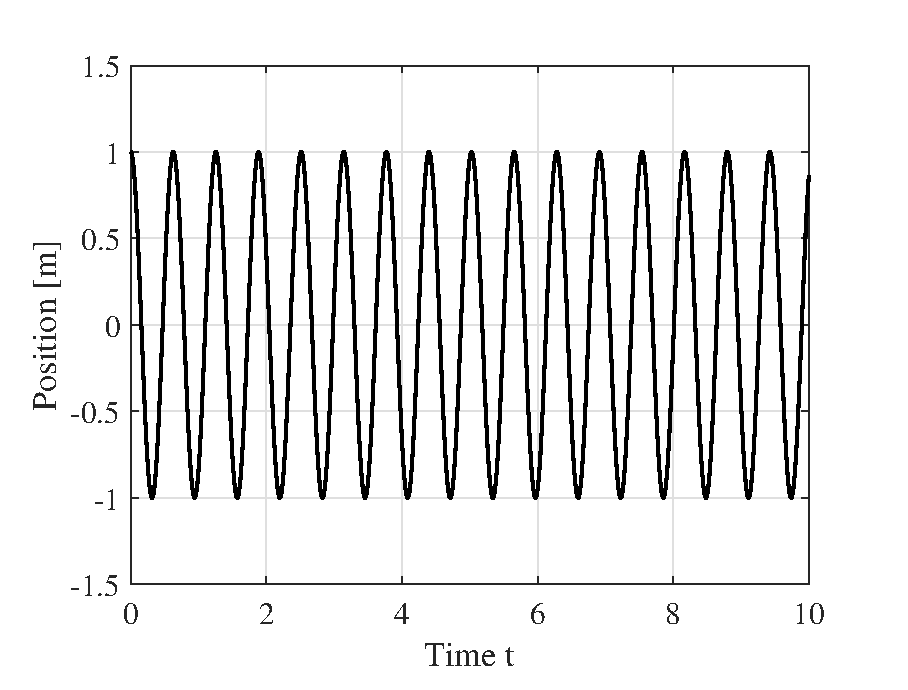
\includegraphics[width=0.33\textwidth]{rungekutta_position.eps}
		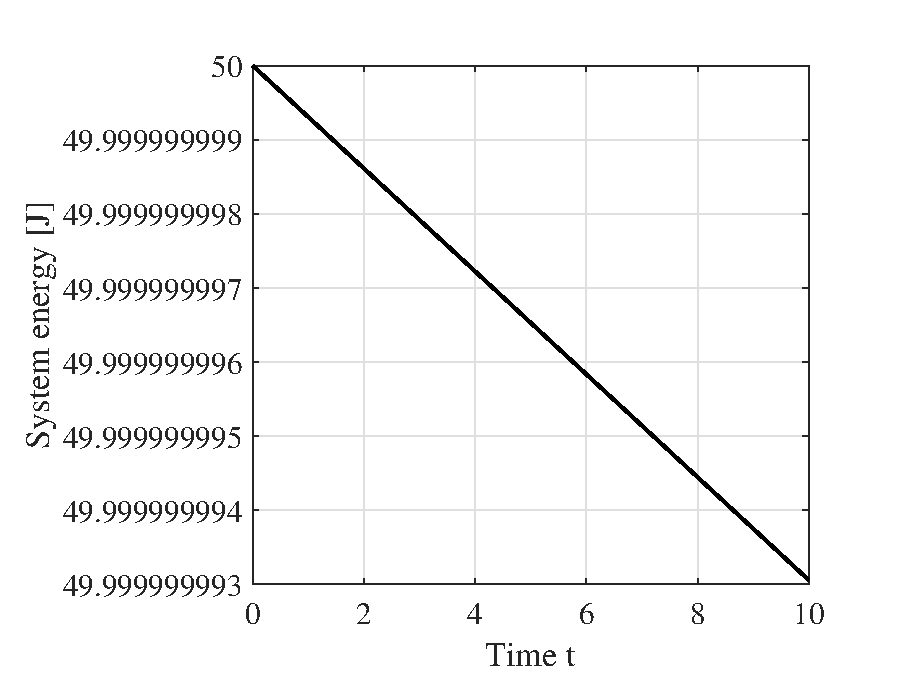
\includegraphics[width=0.33\textwidth]{rungekutta_energy.eps}
		\caption{Mass-spring system with Runge-Kutta method, $\Delta t = 0.001$ s, $m = 1$ kg, $k = 100$ N/m, $A = 1$ m.\label{fig:rungekutta_mass_spring}}
	\end{figure}
	
\end{document}